%\documentstyle[epsf,twocolumn]{jarticle}       %LaTeX2e仕様
%\documentclass[twocolumn]{jarticle}     %pLaTeX2e仕様(platex.exeの場合)
\documentclass[twocolumn]{ujarticle}   %pLaTeX2e仕様(uplatex.exeの場合)
%%%%%%%%%%%%%%%%%%%%%%%%%%%%%%%%%%%%%%%%%%%%%%%%%%%%%%%%%%%%%%
%%
%%  基本バージョン
%%
%%%%%%%%%%%%%%%%%%%%%%%%%%%%%%%%%%%%%%%%%%%%%%%%%%%%%%%%%%%%%%%%
\setlength{\topmargin}{-45pt}
%\setlength{\oddsidemargin}{0cm}
\setlength{\oddsidemargin}{-7.5mm}
%\setlength{\evensidemargin}{0cm}
\setlength{\textheight}{24.1cm}
%setlength{\textheight}{25cm}
\setlength{\textwidth}{17.4cm}
%\setlength{\textwidth}{172mm}
\setlength{\columnsep}{11mm}

%\kanjiskip=.07zw plus.5pt minus.5pt


% 【節が変わるごとに (1.1)(1.2) … (2.1)(2.2) と数式番号をつけるとき】
%\makeatletter
%\renewcommand{\theequation}{%
%\thesection.\arabic{equation}} %\@addtoreset{equation}{section}
%\makeatother

%\renewcommand{\arraystretch}{0.95} 行間の設定
%%%%%%%%%%%%%%%%%%%%%%%%%%%%%%%%%%%%%%%%%%%%%%%%%%%%%%%%
%\usepackage{graphicx}   %pLaTeX2e仕様(\documentstyle ->\documentclass)
\usepackage[dvipdfmx]{graphicx}
\usepackage{subcaption}
\usepackage{multirow}
\usepackage{amsmath}
\usepackage{url}
\usepackage{ulem}
%%%%%%%%%%%%%%%%%%%%%%%%%%%%%%%%%%%%%%%%%%%%%%%%%%%%%%%%
\begin{document}

	%bibtex用の設定
	%\bibliographystyle{ujarticle}
	\twocolumn[
	\noindent

	\hspace{1em}
	2020 年 01 月 10 日
	ゼミ資料
	\hfill
	M1 寺内 光

	\vspace{2mm}

	\hrule

	\begin{center}
		{\Large \bf 進捗報告}
	\end{center}


	\hrule
	\vspace{3mm}
	]

	% ‚ここから 文章 Start!
	\section{今週やったこと}
	マルチモーダルを扱う研究の準備として自然言語処理(特にseq2seqに関わるようなところ)のリサーチをした.\cite{nlp-research} がよくまとまっていて分かりやすかった.

	\begin{itemize}{
		\item{画像キャプション生成}
		\item{transformer, BERT}
		\item{NASセットアップ}
	}
	\end{itemize}

	\subsection{画像キャプション生成}
	画像と自然言語をつなぐ代表的なタスクとして画像キャプション生成があるので調べた.
	図 \ref{fig:captioning} に LSTM を用いた代表的な 4 種類のモデルを示す.

	\begin{figure}[h]
		\centering
		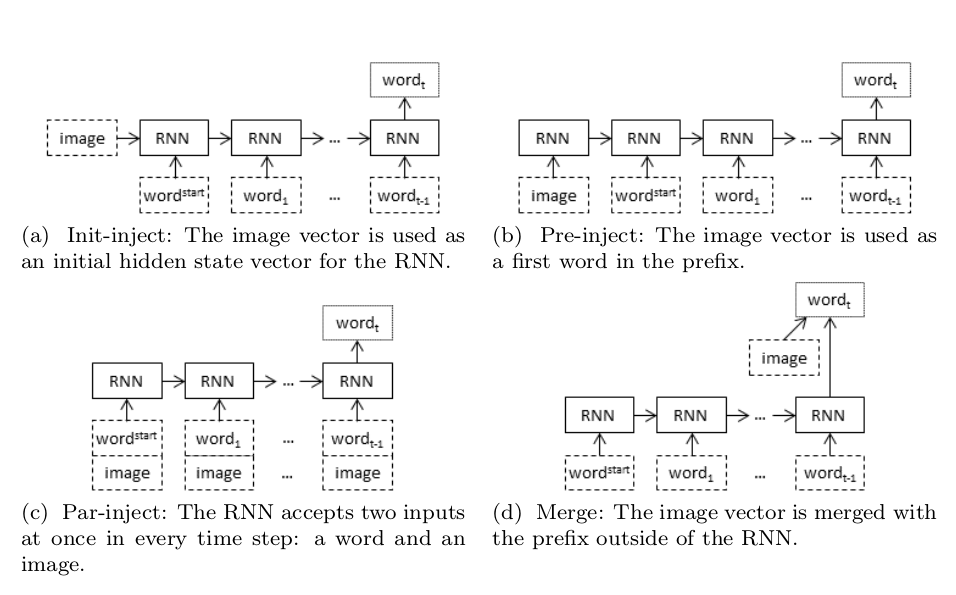
\includegraphics[width=1.0\columnwidth]{1.png}
		\caption{画像キャプション生成における代表的なモデル}
		\label{fig:captioning}
	\end{figure}

	\begin{itemize}
		\item{a:init-inject)}LSTMの隠れ層の初期状態として画像の分散表現を用いる
		\item{b:pre-inject)}画像を入力データの1時系列目として用いる
		\item{c:par-inject)}各時系列に対して画像をconcatして用いる(やや冗長)
		\item{d:merge)}LSTMの出力と画像の分散表現をマージする
	\end{itemize}
	先行研究によると init-inject と merge が良い精度を出している \cite{DBLP:journals/corr/TantiGC17}.

	4コマ漫画をマルチモーダルに LSTM でやろうとするとこのあたりをベースに組むのかなという感じ.
	ひとまずは去年の話題にも上がっていた LSTM を用いないセリフマッチング問題に取り組んでみる.

	\subsection{transformer, BERT}
	そのうちセリフの分散表現をとってくるときにBERTを使うと思うので,原著と論文解説等を読んだ.背景と特徴を押さえつつ従来の Encoder-Decoder モデルと対比しつつ読み,ふんわりとした理解だがアイデアの概要を掴んだ.

	\section{来週の予定}\noindent
	\begin{itemize}{
		\item{4コマ漫画ストーリーデータセットの自然言語データのフォーマット}
		\item{画像と自然言語の分散表現のマッチング試行}
		\item{DCAIの原稿作成(1/31〆)にとりかかる}
	}
	\end{itemize}

	\bibliographystyle{unsrt}
	\bibliography{2020_01_10_terauchi}

\end{document}
